\documentclass[10pt]{article}

%%% These are some packages that are useful
\usepackage{amsmath,amssymb, amscd,amsbsy, amsthm, enumerate}
\usepackage[export]{adjustbox}
\usepackage{lastpage}
\usepackage[top=1in, bottom=1in, left=1in, right=1in]{geometry}
\usepackage[unicode]{hyperref}
\usepackage{tikz, pgfplots, xcolor, fancyhdr}
\usepackage{multicol,caption}
\usepackage{lipsum}
\usepackage[version=4]{mhchem}
\usepackage{float}

%%% Page formatting
%\setlength{\headsep}{30pt}
\setlength{\textheight}{9in}
\newcommand{\tab}{\hspace{1cm}}
%\setlength{\parindent}{25pt}

\title{Deceit Through Statistics}
\author{Antonius Torode}

%%% Header and Footer Info
\pagestyle{fancy}
\fancyhead[L]{{\large Template - \textbf{Change 03}}}
\fancyhead[C]{\today}
\fancyhead[R]{Name: Antonius Torode}


\fancyhf{} % sets both header and footer to nothing
\renewcommand{\headrulewidth}{0pt}
% your new footer definitions here

\fancyfoot[L]{}
\fancyfoot[C]{}
\fancyfoot[R]{\thepage\ of \pageref{LastPage}}

% Used to define spacing and format of References
\let\OLDthebibliography\thebibliography
\renewcommand\thebibliography[1]{
	\OLDthebibliography{#1}
	\setlength{\parskip}{0pt}
	\setlength{\itemsep}{0pt plus 0.3ex}
}

\newenvironment{Figure}
  {\par\medskip\noindent\minipage{\linewidth}}
  {\endminipage\par\medskip}


%%% Document Starts now
\begin{document}

\maketitle
\thispagestyle{fancy}


\begin{abstract}
This message explores the subtle and pervasive nature of deceit as different from lying. It draws on biblical teachings and modern examples to caution the faithful. Using various scriptures, this message examines how deceit operates as a powerful tool of evil, often masquerading as truth. A practical illustration using the PCR COVID-19 tests reveals how a single truthful statement can mislead when context is omitted, paralleling the deceptive allure of end-times Babylon.
\end{abstract}

\begin{multicols}{2}


\begin{quotation}
``Deliver my soul, O Lord, from lying lips \textit{And} from a deceitful tongue.'' - Psalm 120:2 (NKJV)
\end{quotation}

Lying is not the same as deceit. If someone tells you a lie, you may realize it, but if someone deceives you, you will not know. For if you realize it, then you are no longer deceived. Deceit is a tool used by the evil. It's a powerful tool. It allows evil to masquerade as good - as an angel of light. 

\begin{quotation}
``Deceit is in the heart of those who devise evil.'' - Proverbs 12:20 (NKJV)
\end{quotation}

Deception is something that we all need to be aware of. We need to understand that it's all around us, and it's targeting us continually in our everyday lives. But deceit is not something which is always easy to catch. Sometimes, it appears as kind, genuine, or even as something obvious and trustworthy. That is why deception is such a powerful tool.  

\begin{quotation}
``He who hates, disguises \textit{it} with his lips, And lays up deceit within himself. When he speaks kindly, do not believe him, For \textit{there are} seven abominations in his heart; \textit{Though his} hatred is covered by deceit.'' - Proverbs 26:24-26 (NKJV)
\end{quotation}

Consider the end time Babylon. A great city which reigns over the kings of the earth\footnote{Revelation 17:18 - ``And the woman whom you saw is that great city which reigns over the kings of the earth.''}. A city of gold and precious stones - clothed in fine linen, purple, and scarlet. But how does Babylon get this way?

\begin{quotation}
``The light of a lamp shall not shine in you anymore, and the voice of bridegroom and bride shall not be heard in you anymore. For your merchants were the great men of the earth, for by your sorcery all the nations were deceived.'' - Revelation 18:23
\end{quotation}

By her sorcery, all the nations will be deceived. But what is sorcery? The word `sorcery' here is the greek word \textit{pharmakeia} \cite{pharmakeia}. Pharmakeia is commonly translated to \textit{sorcery} or \textit{witchcraft}, but the Lexical definitions from Bible concordances are as follows:
\begin{enumerate}\itemsep0em 
\item the use or the administering of drugs.
\item poisoning ("pharmacy").
\item (metaphorically) the deceptions and seductions of idolatry.
\end{enumerate}
With everything we know about Babylon, the third definition likely fits the best, but all three of these would fit in some way, shape, or form. The first two definitions are used as a metaphor for the third. Thus, you can gleam a lot by expanding on them. Drugs are very much a way of seducing. They can make you feel better and forget about worldly pains. Drugs are very much a form of idolatry. So are drugs a tool of deception? I'm not going to say that the drug industry is what  Revelation 18:23 is referring to - that is up for interpretation. I am, however, going to use the drug industry as an example to demonstrate the scale, reach, and recurring pattern of deception. It serves as a practical example to show the power of deception.

First, drugs and pharmaceuticals have a truly global impact. According the the U.S Justice department, in 2009, the company Pfizer was ordered to pay a \$2.3 \textit{billion} fine for fraudulent marketing \cite{pfizer_fine}. As the press release put it, they had to pay ``the largest criminal fine ever imposed in the United States for any matter.'' This was for the sale of a \textit{single} drug. This is just one of many incidents like this, and as we all know from recent experiences, Pfizer is very much a functioning and active corporation. This demonstrates the vast scale that the drug companies operate at - which is a truly global influence. It is therefore not too hard to believe that this industry could be capable of affecting the entire world. But what about deceiving it?

Through a simple statistical example, it can be seen just how easy it is to deceive. This example is demonstrated by applying something called Bayes Theorem\footnote{For those not mathematically inclined, a theorem is a statement that has been proven to be true using logic and previously established facts. Although similar sounding, it is \textit{not} a `theory'.}. This example will be somewhat simplified, but hopefully demonstrates clearly how easy it is to deceive through statistics. 

This example begins with a simple statement:
\begin{quotation}
``The rapid Polymerase Chain Reaction (PCR) COVID test is 95\% accurate!''
\end{quotation}
Assume this statement is completely true. There is no lying here - just a simple statement of fact. This statement alone would give you great confidence in the PCR test. If you got tested for COVID using this test, the results should be quite accurate, because it is indeed `95\% accurate!' So therefore, if you were to take one of these tests, and it gave you a positive result (meaning the test thinks you have COVID), what's the likelihood that you actually have COVID? Well, most reasonable people might conclude that there's a 95\% chance you have COVID. That seems reasonable. However, even a test that's 95\% accurate can mislead us when the disease is rare, as a simple calculation shows.

Let us now setup a scenario. Suppose we have a disease, say COVID, which infects about 10 people per 100,000 people at any given moment (that's almost a million people at any given time), which is the number reported by TIME magazine in June of 2020 \cite{TIME}. What that means is that if you take 100,000 random people, 10 of them will be infected with COVID. This was around the same time that PCR was being rolled out to test \textit{everyone}. So then what would happen if you did test everyone?

Recall that the PCR test we're using is 95\% accurate. Which means if we test someone, there's a 95\% chance that the result will be accurate. So let us take our group of 100,000 random people and test every single one of them. We begin testing them one by one, and each test is 95\% accurate. For the sake of argument, let's say all 10 people who are infected give an accurate result (hooray). But as we test those who are not infected, we get an incorrect result 5\% of the time. This means that 5\% of the people in our group of 100,000 will have incorrect results. Therefore, there will be about 5,000 people who test \textit{positive}, even though they do \textit{not} have COVID. But the other 95,000 people will have tested accurately. That seems like good odds, until you re-ask the question - what's the likelihood that you actually have COVID? There were 10 people with COVID who tested positive, and then 5,000 people without COVID who also tested positive. Therefore, if you are in that group with a positive test, there is only a $\frac{10}{5010} \approx 0.2\%$ chance that you \textit{actually} have COVID (visually represented in Figure 1)! And that is when using a test which is 95\% accurate! This shows how truthful statements, like '95\% accurate,' can deceive when context is omitted, mirroring how evil can masquerade as good.

\begin{Figure}
	\centering
	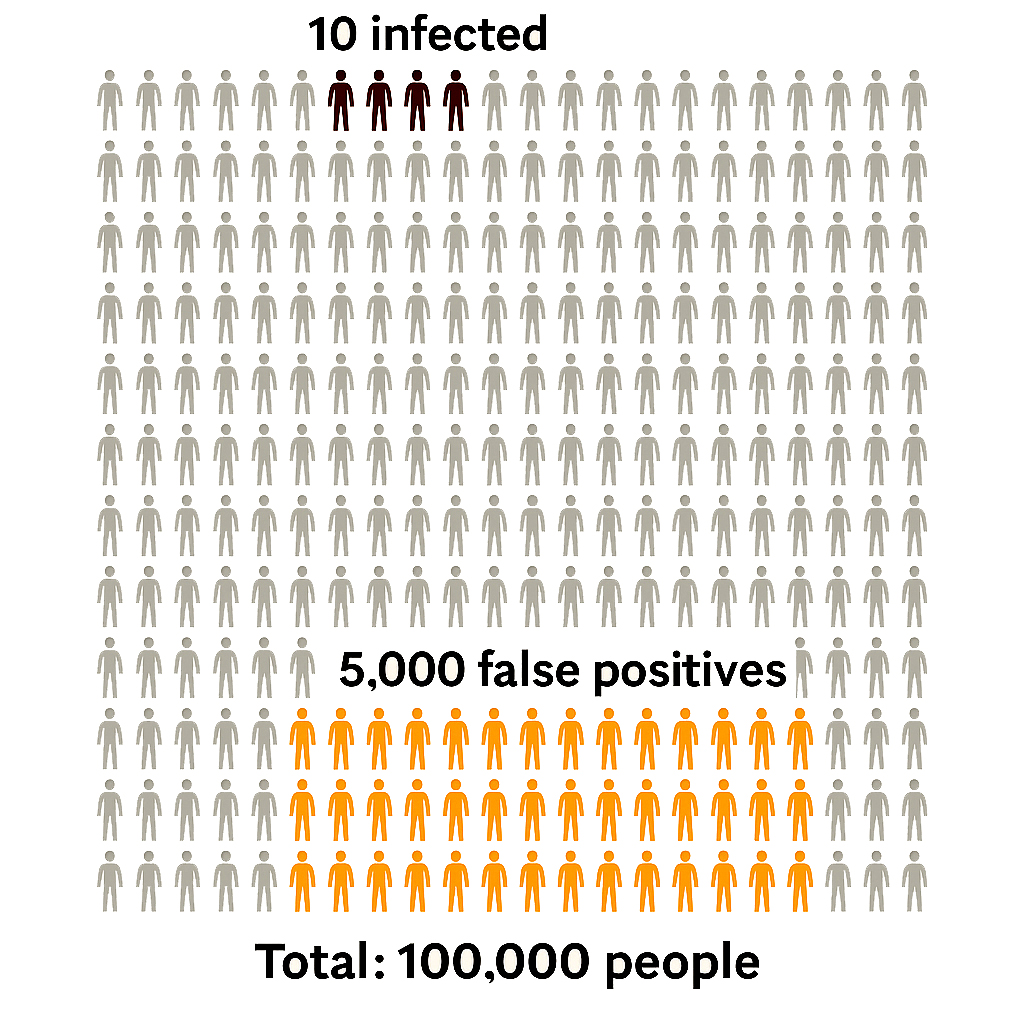
\includegraphics[width=\textwidth]{infection_diagram.jpg}
	{\footnotesize Figure 1. This diagram visually represents Bayes Theorem. While it does not show exactly 100,000 individuals, 10 infected cases, or 5,000 false positives, it illustrates the dramatic contrast between true positives (black) and false positives (orange) when testing a large population with a low infection rate, even when using a test with 95\% accuracy.}
\end{Figure}

This is just a single example among many. It demonstrates that by telling a single truth, you can plant a seed which can grow to fool the nations. Deceit is a tool far greater than lies. Deceit uses the truth to lull us into the pleasures of Babylon. Although this example using the sorcery of the earth is just a metaphor, it perfectly demonstrates the dangers around us. Therefore, be vigilant, wise, and cautious. Ask God to deliver you from a deceitful tongue.

\end{multicols}

\begin{thebibliography}{9}
	{\footnotesize
		
		\bibitem{pharmakeia} \url{https://biblehub.com/greek/5331.htm}
		
		\bibitem{godrules} \url{https://godrules.net/library/strongs2b/gre5331.htm}
		
		\bibitem{pfizer_fine} ``Justice Department Announces Largest Health Care Fraud Settlement in Its History.'' 9/2/2009. \url{https://www.justice.gov/archives/opa/pr/justice-department-announces-largest-health-care-fraud-settlement-its-history}
		
		\bibitem{TIME} ``The U.S. Has Officially Unflattened the Curve With Its Worst Day of the Coronavirus Pandemic Yet.'' 6/25/2020. \url{https://time.com/5859796/coronavirus-us-worst-day/?utm_source=chatgpt.com}
		
	}
\end{thebibliography}


%%%%%%%%%%%%%%%%%%%%%%%%%%%%%%%%%%%%%%%%%%%%%%%%%%%%%%%%%%%%%%%%%%%%%%%%%%%%%%%%%%%%%%%%%%%
\end{document}





















}{den}
